\section{Simulation and analysis methodology.}

First an initial ($\la_0$) and final control parameter $\la_f$ are chosen, then integration step is chosen to be a fourth of the smallest expected time-scale for the autonomous system. 
In this case, for 1-dimensional systems, the smallest time-scale is chosen as $t_{min}=min (-1/2M)$ chosen as $1/2M$ since the stochastic timescale from \cref{eq: ST_variance}  instead of $1/M$, therefore this is set by the most stable point of the system\footnote{In appendix \ref{apx:param_speed_integration} an intuitive scheme is presented on why this choices of time step are also relevant for the stability of the numerical integration.}. 

Rewriting the criteria of \cite{Thompson2011a} for the windowing  and separation of scales\footnote{In \cite{Thompson2011a} the sweeping rate is, called drift rate in their paper ($\kappa_{\mathrm{drift}}$) , is defined as the average sweeping rate  of the control parameter. However this rate will have the units of the control parameter per second, while our definition has units of $1/s$ as does the LDR.}, as timescales:
\begin{equation}
	\int \frac{d\la}{c_\la} >> -\frac{1}{||M||}>> -\frac{1}{M_{\mathrm{other-scales}}}
\end{equation}
where $M_{\mathrm{other-scales}}$ refers to the other eigenvalues $m$ when the system has more dimensions. This equivalent to asking for a clear separation of timescales in the deterministic backbone, and a clear separation of timescale with the sweeping parameter that is equivalent to a slow sweeping rate. 
As we have shown, this relations can only hold far from the critical bifurcation, since no matter how it is approached, at some point the sweeping rate will be similar and then smaller than the relaxation time\footnote{Unless it is possible in some scenario to slow down the sweeping rate faster than the decay of $M$, though that case the bifurcation point will never be reached.}. 	
	
where the sampling time of the data, $\Delta t_{\mathrm{sample}}$, has to obey
\begin{equation}
	-\frac{1}{||M||} >> \Delta t_{\mathrm{sample}} >> -\frac{1}{M_{\mathrm{other-scales}}}.
\end{equation}



For the analysis, three other scales have to be chosen. A time length for the EWS signal running window calculation; and, in case of using a detrending, a scale for the running detrending window and a bandwidth for the Gaussian kernel of the detrending window. 
Since at the critical bifurcation, the auto-correlation converges to one, the correlation length diverges. 
Therefore, any analysis window close enough to the bifurcation will be too small.

So as before, any windowing we choose can only hold for a range of parameters at some distance to the bifurcation

The detrending for the analysis of the EWS is done by a moving average with a gaussian kernel with bandwidth ($\mu$), such that:
\begin{equation}
	\int \frac{d\la}{c_\la} >> \mu >> -\frac{1}{||M||}
\end{equation}
and the EWS analysis window
\begin{equation}
	\int \frac{d\la}{c_\la} >> (2m+1)\Delta t 
\end{equation}

In particular we choose
\begin{equation}
	-\frac{1}{2||M||} >> \Delta t_{\mathrm{sample}}  
\end{equation}
 since this is the time-scale for the noise.
 
This definitions are consistent with the influence of the sweeping parameter speed, since all the analysis windows are dependent of this factor. 
Therefore, it is important to state this scales compared to the sweeping time-scale (when possible) since the same analysis windows are not easily compared for examples with a different control parameter speed.

All simulations are made following the same criteria, unless specified otherwise.

\section{examples:}
Models by review: 
\cite{Dutta}: Multiplicative noise.

Saddle fold. Transctitical, supercritical, pitchfork, bif wthout CSD, No transition, Sharp transition.



\subsection{Custom (change name)}

A first step towards a more complex study case, would be to add more equilibria to the bifurcation of $\dot{x}=-\lambda x$. A simple way to do this is to add two other equilibria around the $x^*=0$. 

\begin{equation}
	\begin{cases}
			dx &=\lambda(x)(x-1)(x+1)\, dt +\sigma \, dW\\
		d\la&=c_\la \, dt
	\end{cases}
	\label{eq:ASScustom}
\end{equation}

Now the equilibria are  $x^*=\left\lbrace -1,0,1 \right\rbrace $. In this system there is no deviation due to the linear lag since $d_\la x^*=0$. 


\begin{figure}
	\centering
	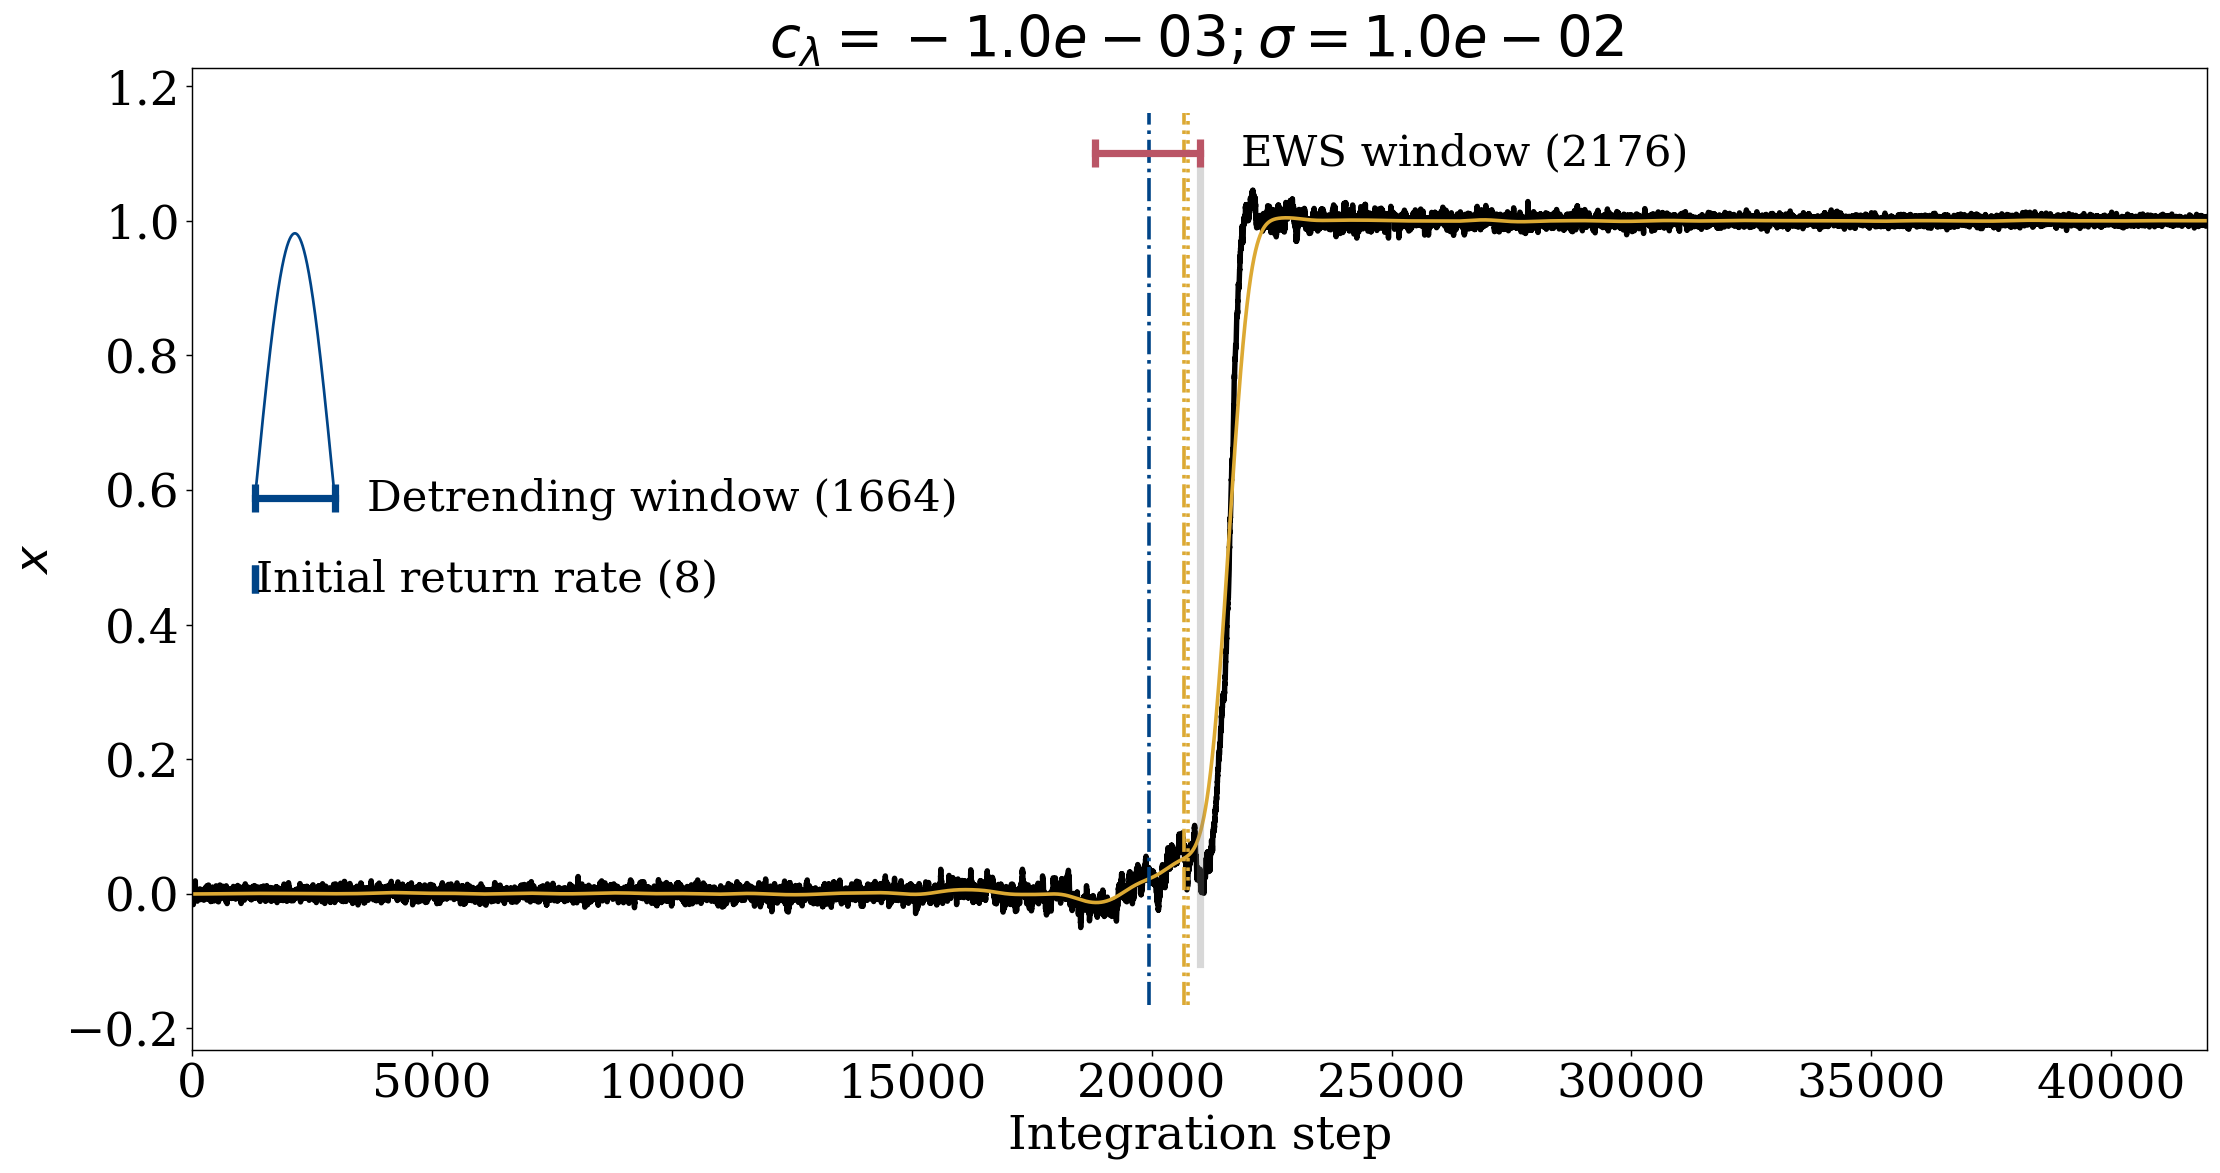
\includegraphics[width=0.8\linewidth]{Images/Metrics/custom_bifurcation/detrend_additive}
	\caption{}
	\label{fig:detrendadditive}
\end{figure}

\begin{figure}
	\centering
	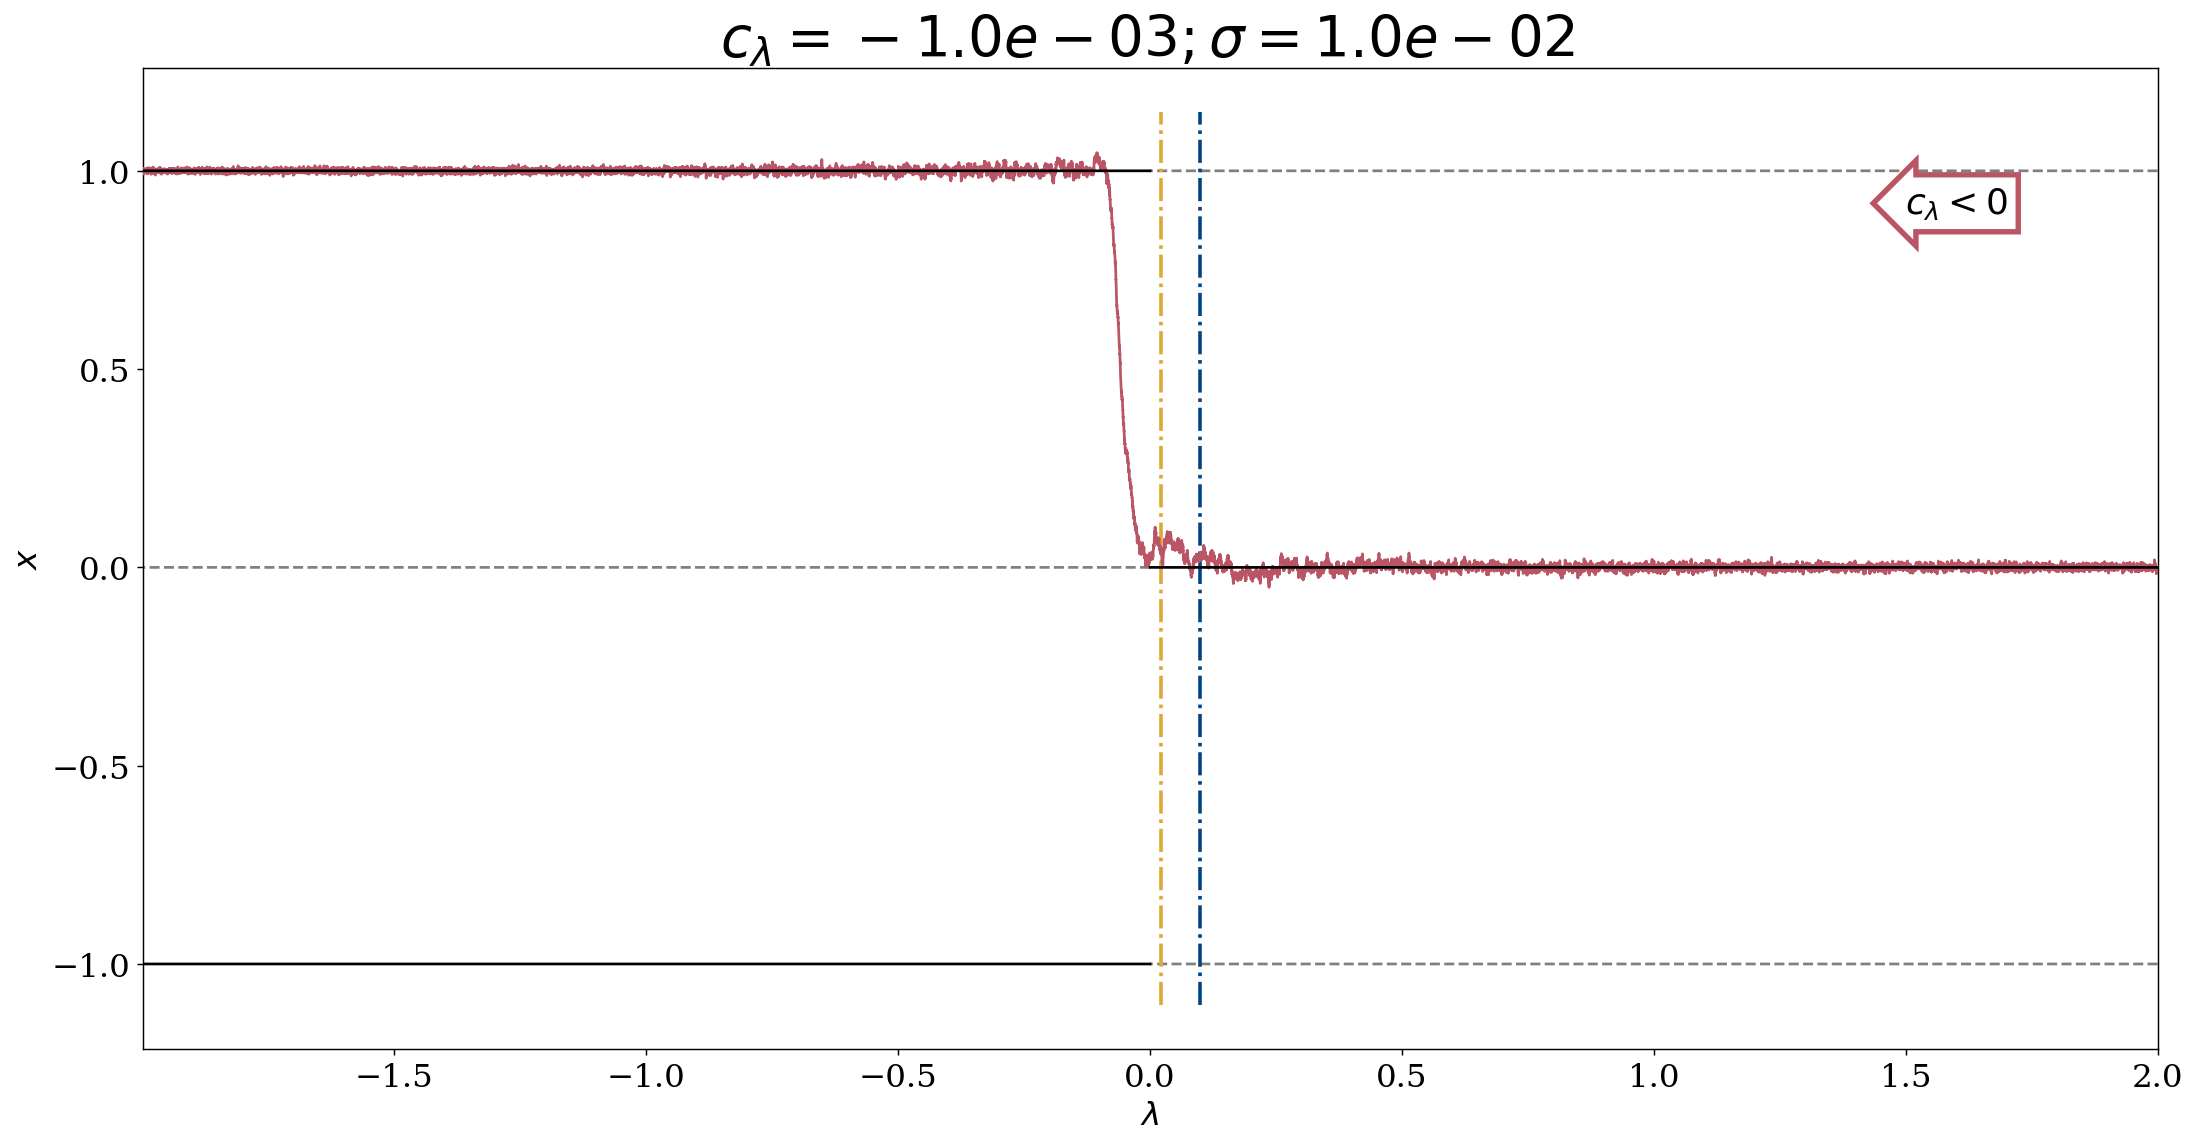
\includegraphics[width=0.8\linewidth]{Images/Metrics/custom_bifurcation/bifurcation_additive}
	\caption{}
	\label{fig:bifurcationadditive}
\end{figure}


\begin{figure}
	\centering
	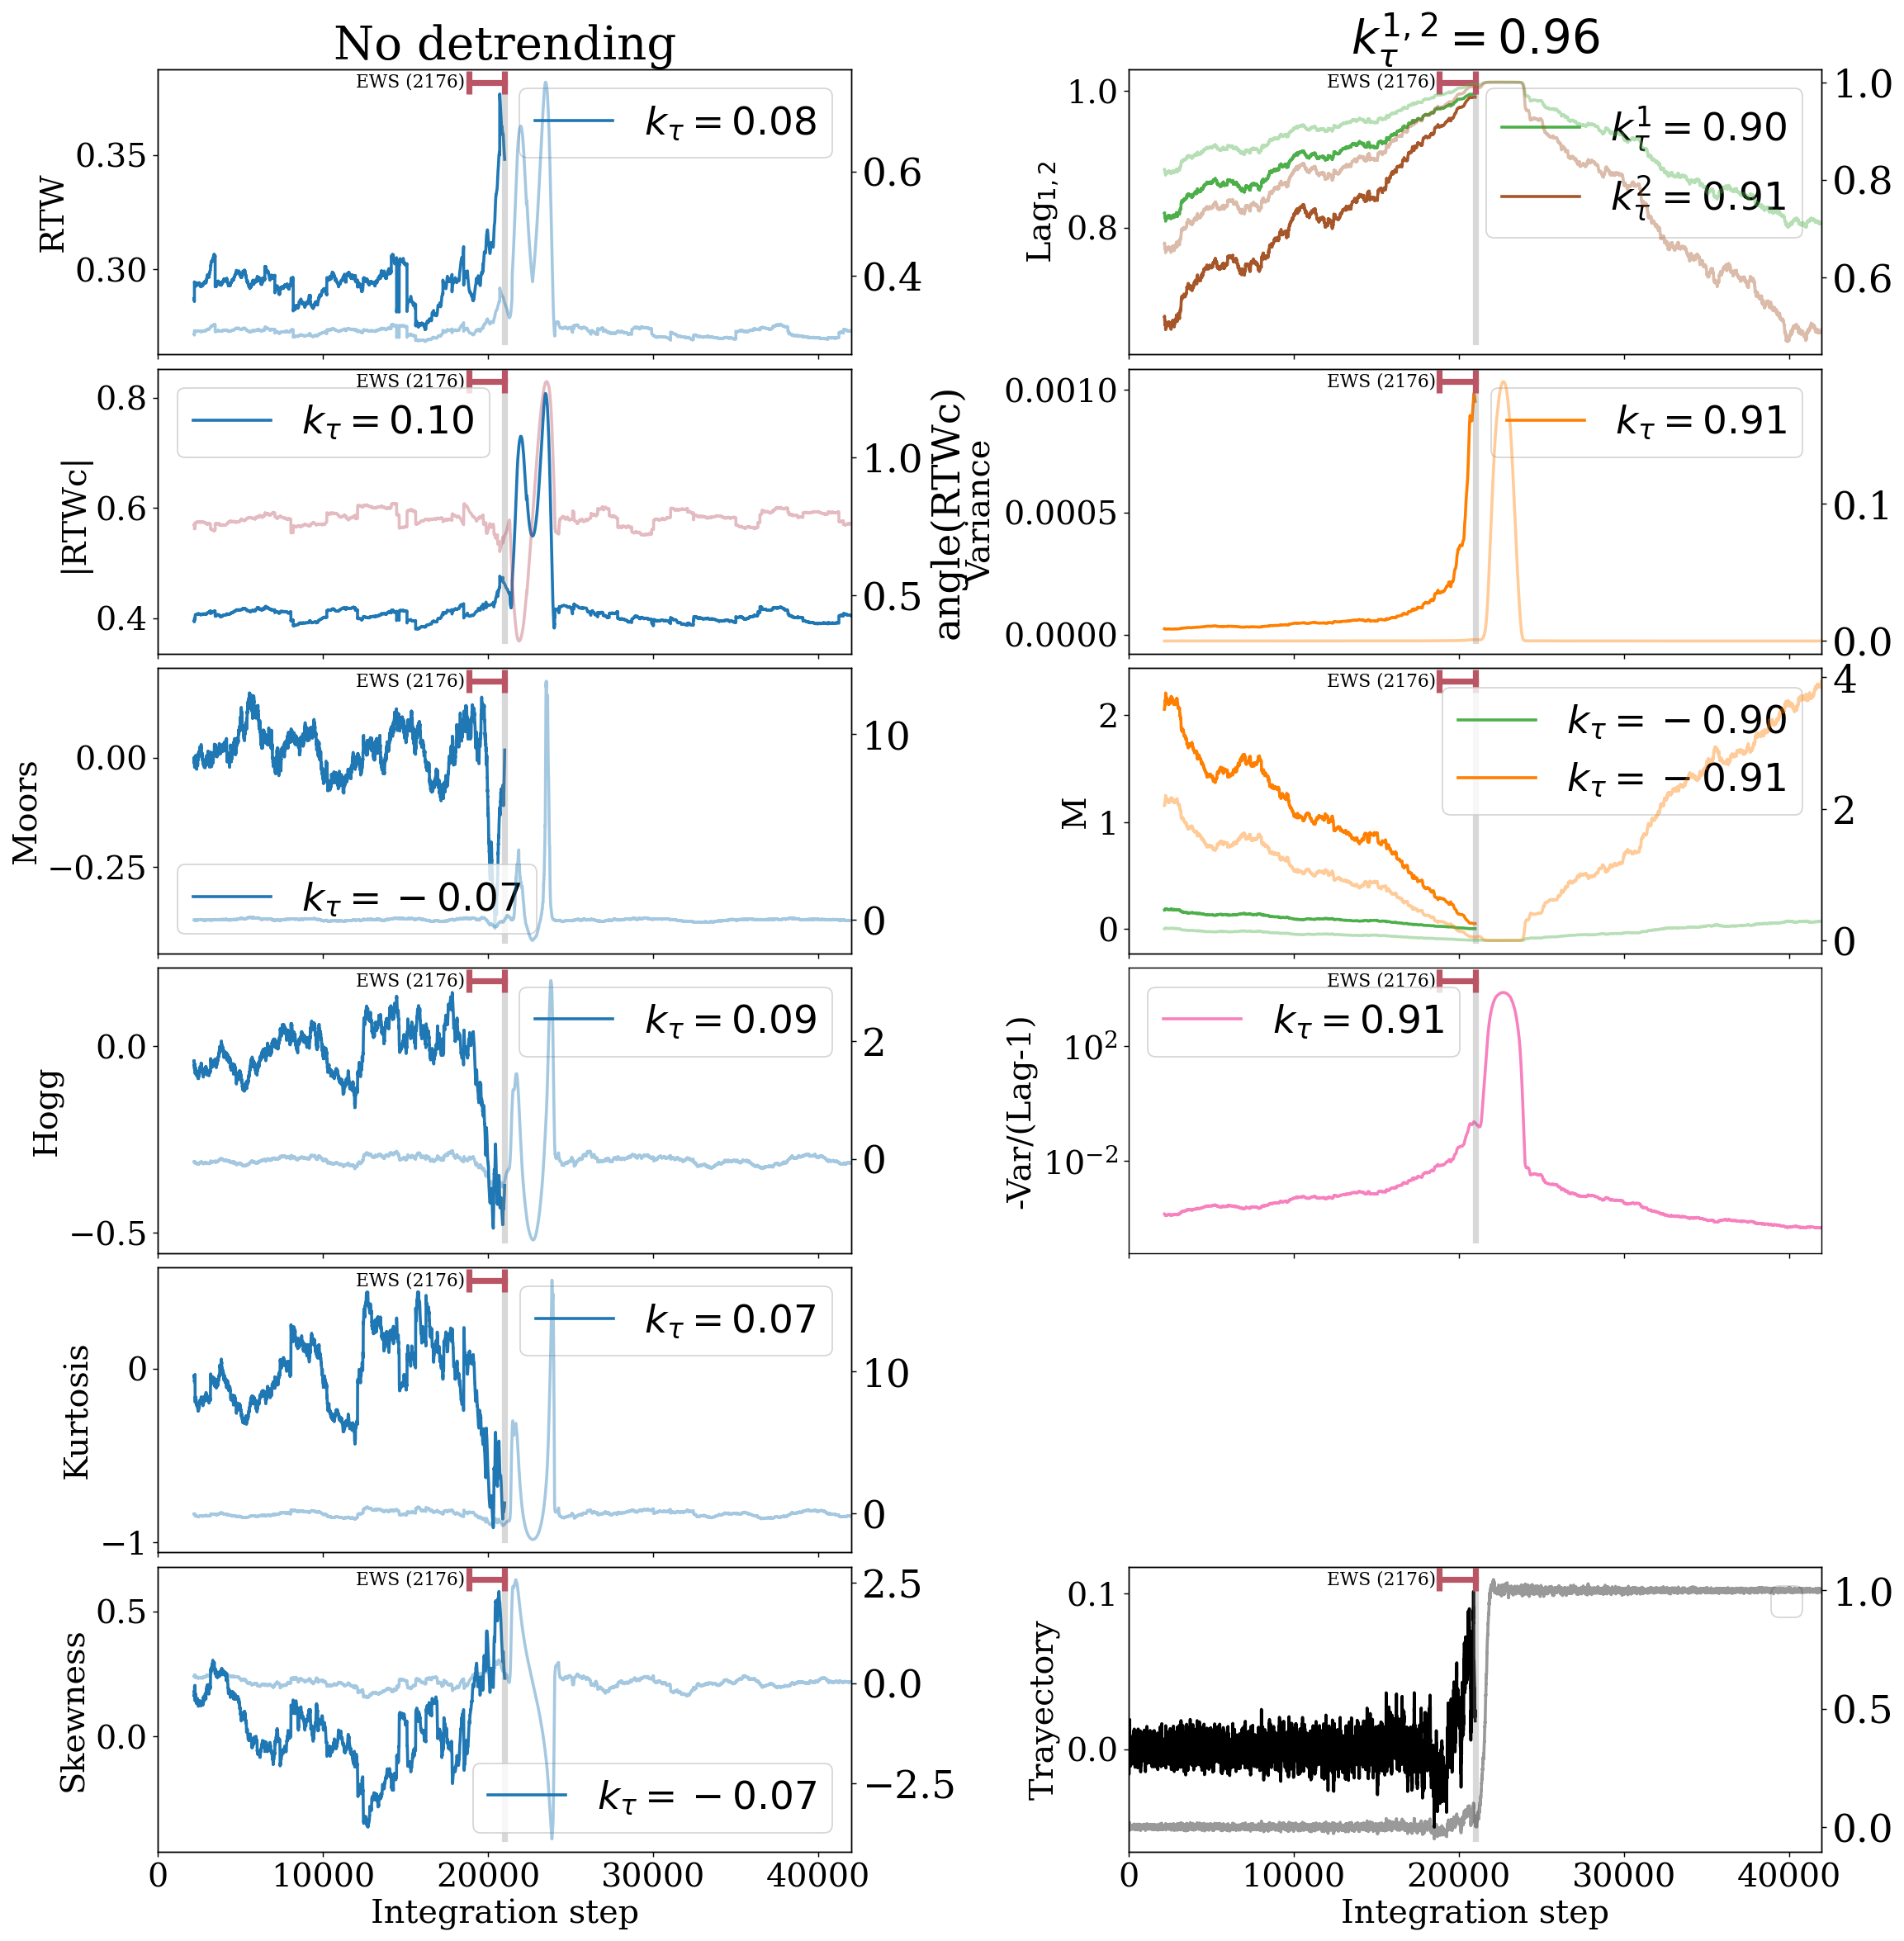
\includegraphics[width=0.8\linewidth]{Images/Metrics/custom_bifurcation/No_det_additive}
	\caption{}
	\label{fig:nodetadditive}
\end{figure}
\begin{figure}
	\centering
	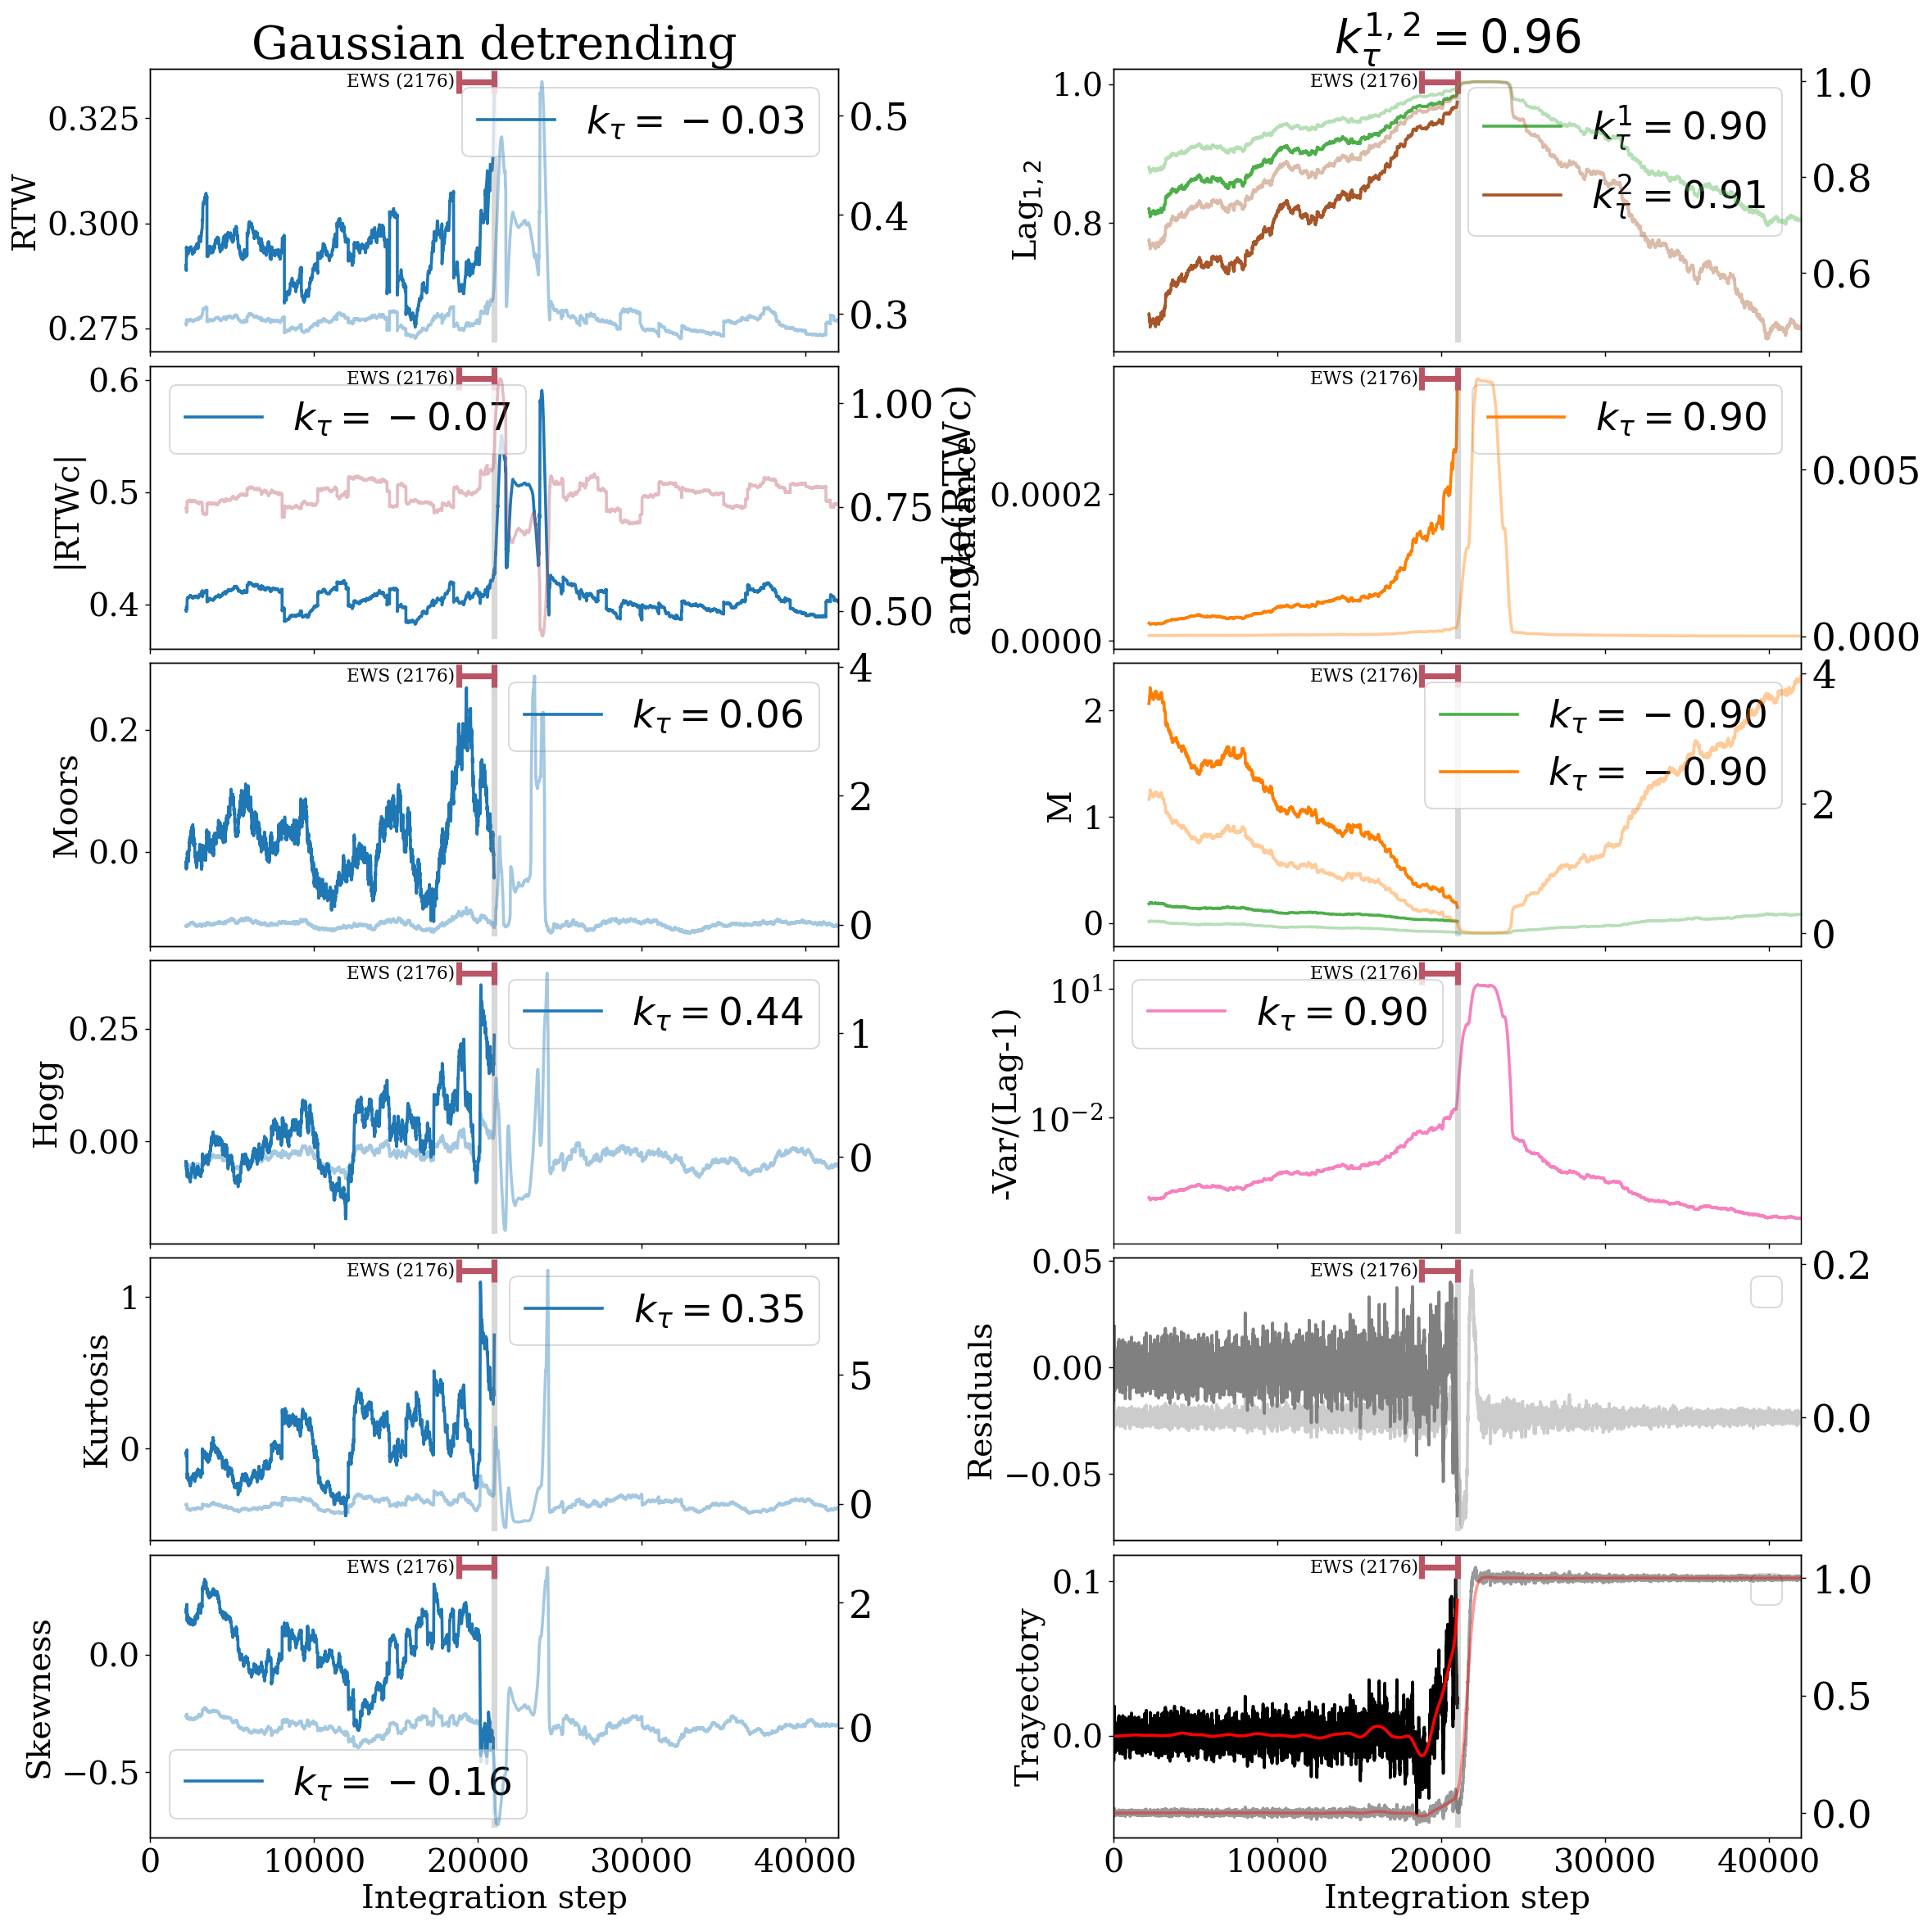
\includegraphics[width=0.8\linewidth]{Images/Metrics/custom_bifurcation/Gdet_additive}
	\caption{}
	\label{fig:gdetadditive}
\end{figure}





\subsection{Sub-critical pitchfork}



\begin{equation}
	\begin{cases}
	dx&=(\lambda x+x^3-x^5) \, dt +\sigma \, dW\\
		d\la&=c_\la \, dt
	\end{cases}
	\label{eq:ASSsubcri_pitch}
\end{equation}



\subsection{Super-critical pitchfork}

\begin{equation}
	\begin{cases}
		dx&=(\lambda x+x^3) \, dt +\sigma \, dW\\
		d\la&=c_\la \, dt
	\end{cases}
	\label{eq:ASSsupercri_pitch}
\end{equation}

This system has three fixed points, $x={0,\pm \sqrt{1/2}\sqrt{1\pm\sqrt{1+4\lambda }}}$



\subsection{Abundance}
	$b=1$,$r=1$
\begin{equation}
	\begin{cases}
		dN&=(rN(1-N/K)-\la \frac{N^2}{N^2+b^2}) dt +\sigma \, dW\\
		d\la&=c_\la \, dt
	\end{cases}
	\label{eq:ASSabun}
\end{equation}

\subsection{Hopf  bifurcation}

\begin{equation}
	\begin{cases}
		dN&=(rN(1-N/\la)-a \frac{N P}{N+b}) dt +\sigma_1  \, dW\\
		dP&=\frac{eaNP}{(b+N)-dP} dt +\sigma_2  \, dW\\
		d\la&=c_\la \, dt
	\end{cases}
	\label{eq:ASSabun_hopf}
\end{equation}



\begin{equation}
	\begin{cases}
		dx&=(\la (x-\la)+(x-\la)^3-(x-\la)^5)dt +\sigma \, dW\\
		d\la&=c_\la \, dt
	\end{cases}
	\label{eq:ASSslanted}
\end{equation}


\subsection{Fold bifurcation}


\begin{equation}
	\begin{cases}
		dx&=(-x^2+cx+\la) dt +\sigma  \, dW\\
		d\la&=c_\la \, dt
	\end{cases}
	\label{eq:ASSfold}
\end{equation}

\subsection{Sharp transition (1) }

In this case, since there is no critical transition, we can choose to be 'slow' though the whole evolution, the only important variable is the separation between the time scale of the control parameter and the timescale of the LDR.
 
\begin{equation}
	\begin{cases}
	dx&=-(x-\mathrm{erf}(10\lambda)) \, dt +\sigma \, dW\\
	d\la&=c_\la \, dt
\end{cases}
\end{equation}



\begin{figure}
	\centering
	\includegraphics[width=0.7\linewidth]{"Images/Metrics/sharp transition/bifurcation_additive"}
	\caption{}
	\label{fig:bifurcationadditive}
\end{figure}
\begin{figure}
	\centering
	\includegraphics[width=0.7\linewidth]{"Images/Metrics/sharp transition/detrend_additive"}
	\caption{}
	\label{fig:detrendadditive}
\end{figure}
\begin{figure}
	\centering
	\includegraphics[width=0.7\linewidth]{"Images/Metrics/sharp transition/Gdet_additive"}
	\caption{}
	\label{fig:gdetadditive}
\end{figure}
\begin{figure}
	\centering
	\includegraphics[width=0.7\linewidth]{"Images/Metrics/sharp transition/No_det_additive"}
	\caption{}
	\label{fig:nodetadditive}
\end{figure}

sharp 2
%r*x[0]*(1-x[0]/K)-l*x[0]*2/(b**2+x[0]**2)